\chapter{Bell 202 Demodulation Techniques}
There are a few primary approaches to demodulating 1200 baud 1200Hz/2200Hz AFSK signals in hardware.  However, before talking about the techniques for doing AFSK demodulation, it is worth specifying what type of FSK Bell 202 is. There are two features that are relevant for taking into consideration when demodulating the signal. First is that it is asynchronous, meaning that there is no separate clocking signal and the clocking is embedded within the data signal, hence the conversation on bit stuffing and clocking energy in the APRS Background chapter. If it were synchronous, there would be two different signals coming into the demodulator (which would be the data carrying signal and a clocking signal). The second characteristic is that the FSK is coherent or continuous. This means that there is a continuous signal at bit boundaries and there are no jumps as the signal changes from one frequency to another as seen in Figure \ref{coherentFSKExample} as opposed to non-coherent Figure \ref{noncoherentFSKExample} which does have these jumps. Another name sometime applied to this method of FSK, coherent FSK, is continuous-phase frequency shift keying or CPFSK\,\cite{WikipediaCPFSK}.

\begin{figure}
	\centering
	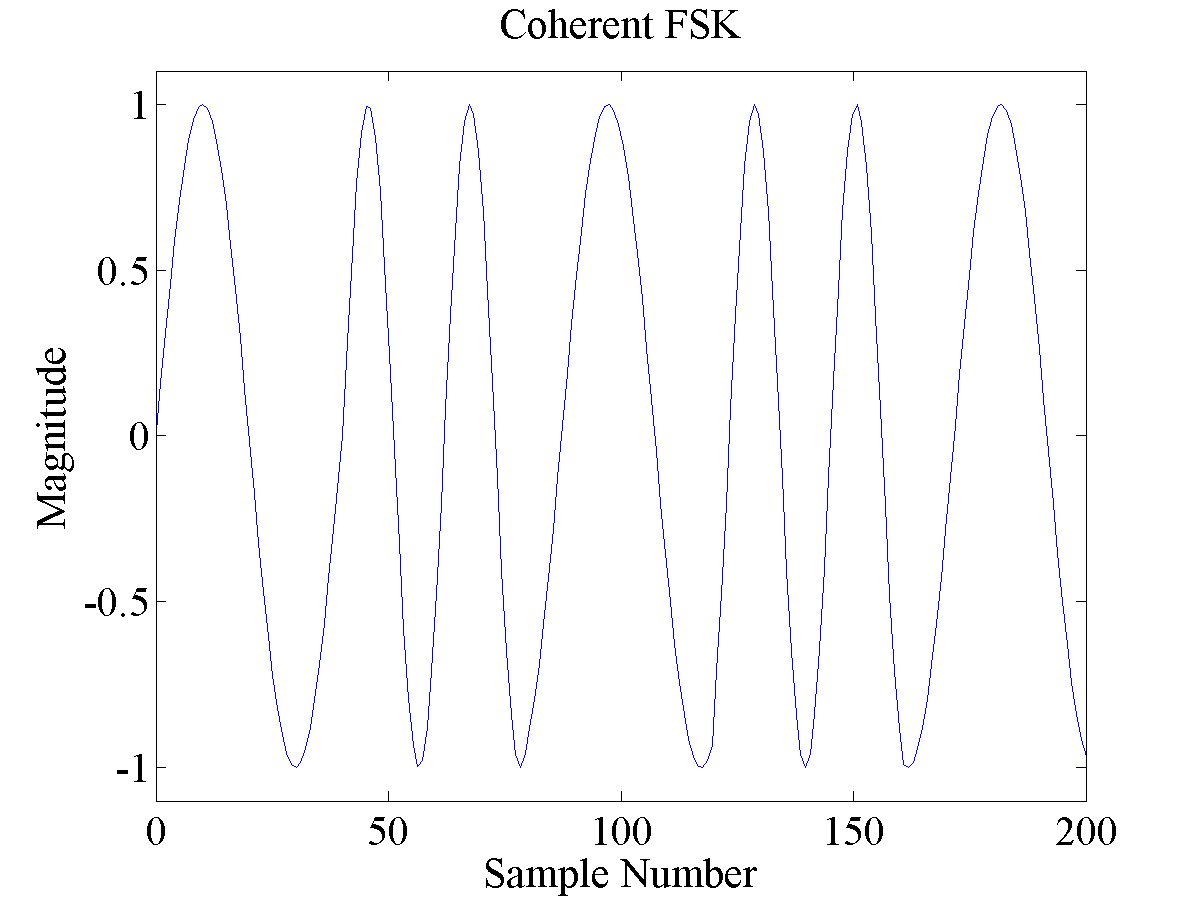
\includegraphics[width=0.75\linewidth]{images/CoherentFSK.png} 
	\caption{Example of a coherent FSK signal.}
	\label{coherentFSKExample}
	\vspace{15mm}
	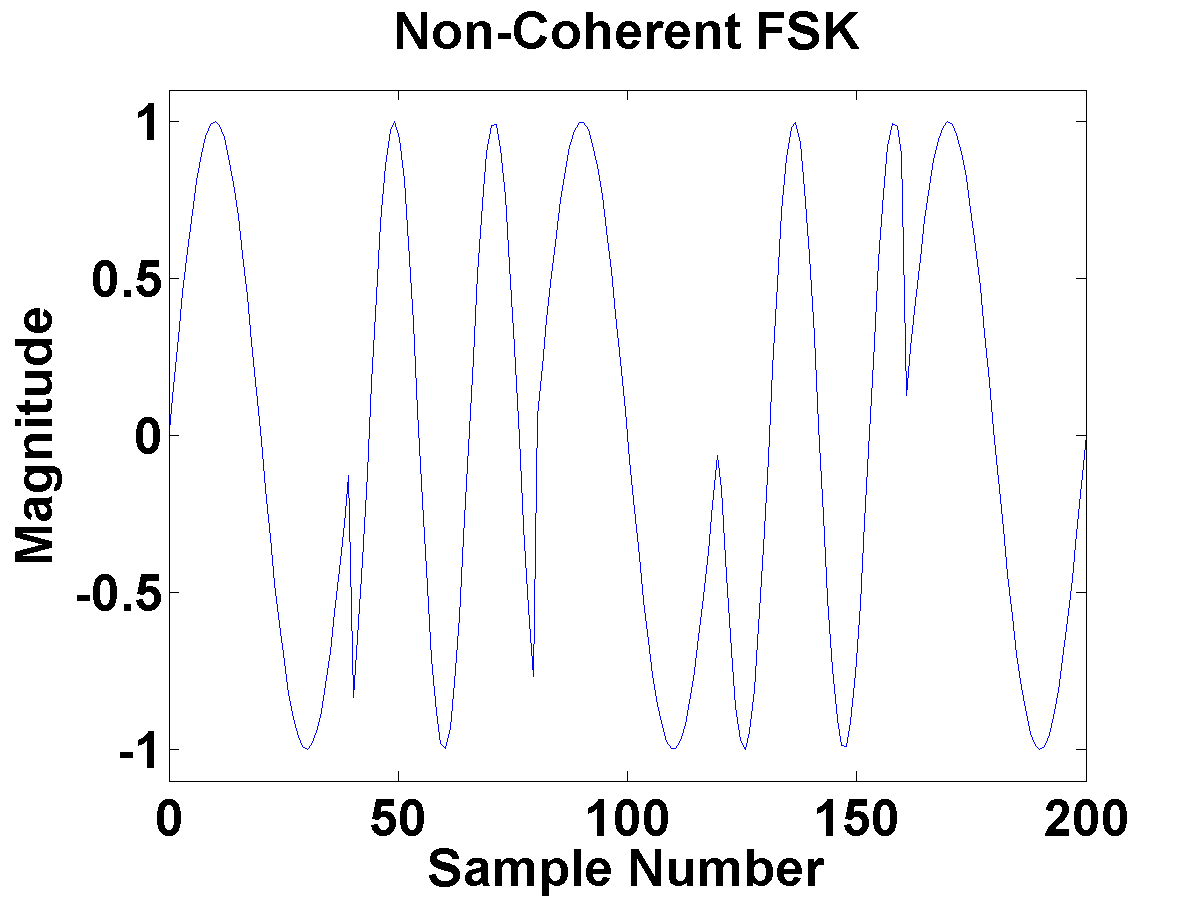
\includegraphics[width=0.75\linewidth]{images/NonCoherentFSK.png} 
	\caption{Example of a non-coherent FSK signal.}
	\label{noncoherentFSKExample}
\end{figure}

Among the demodulation techniques for coherent FSK are edge detection, correlation, filtering, and phase-locked-loops (PLLs). Each of these will be explained in more detail in the corresponding sections below; however with Correlation and Filtering being very popular and mentioned in many books and applications, there is a lot of overlap so more detailed information can be found in the following references\,\cite{MarvinK.Simon1995,Sklar1988,J.Das1986,Proakis1983,Seguine2006,Semiconductor}. The following sections in this chapter explain how the demodulation approach works with the software implementation details being saved for the Implementation chapter. However, there will be an additional section at the end of this chapter to discuss some of the potential advantages of using software over hardware.

\section{Edge Detection}
An edge detection, or zero-crossing, demodulator identifies rising and falling edges in the signal to determine the frequency present. In the TCM3105 chip, which is an FSK modem, rising and falling edges trigger pulses that are at a frequency that is double the input frequency\,\cite{Instruments1994}. Although this is how it is done in hardware, it may be easier to understand through the more simple discussion of zero-crossings. The idea is that based off of the time elapsed between zero crossings (rising and falling edges or vice versa) of the signal, one-half the period of the waveform can be measured. Once the period has been measured the frequency can then be easily calculated using the inverse relationship between period and frequency, \textit{f} = 1 /T where \textit{f} is the frequency and T is the period\,\cite{Seguine2006}. Just to reiterate, two consecutive zero crossings is only half of the period do to the nature of sinusoidal signals. As the TCM3105 is an older chip, a replacement is now commonly used in 1200 baud modem projects, and that is the MX614 made by MX-COM\,\cite{Mitrenga2000}.

\section{Correlation}
A correlation demodulator works through correlating - comparing - an FSK signal with the possible options based off the modulation scheme. In this instance we expect the signal to be either a 1200Hz or 2200Hz signal and hence the signal will be compared to two internal oscillators, one at each frequency\,\cite{Rowe2014}. In practice, the input signal is mixed with each one of the two reference signals and then integrated. The results from each of these correlations is then fed into a decision unit. The output of the decision unit is whichever of the frequencies has more power and hence was more prominent in the signal. The basic block diagram can be seen in Figure \ref{BlockDiagrams}. Correlation is the current method used in Toledo's javAX25. An alternative implementation of a correlator is to have a delay line instead of an internal oscillator. This delay line can delay the input by the time for one period of an expected frequency (i.e. 1/2200Hz) to elapse and then this delayed signal can be multiplied by the original signal\,\cite{Seguine2006}. Essentially, the delayed signal becomes the internal oscillator in this example (see Figure \ref{TimeDelayCorrelator}). Side note, this would work better for higher frequencies than those here since the delay line would be about 145 miles long if using copper wire for the 1200Hz tone\,\cite{HowFastIsElectricity}.

\begin{figure}
  \centering
	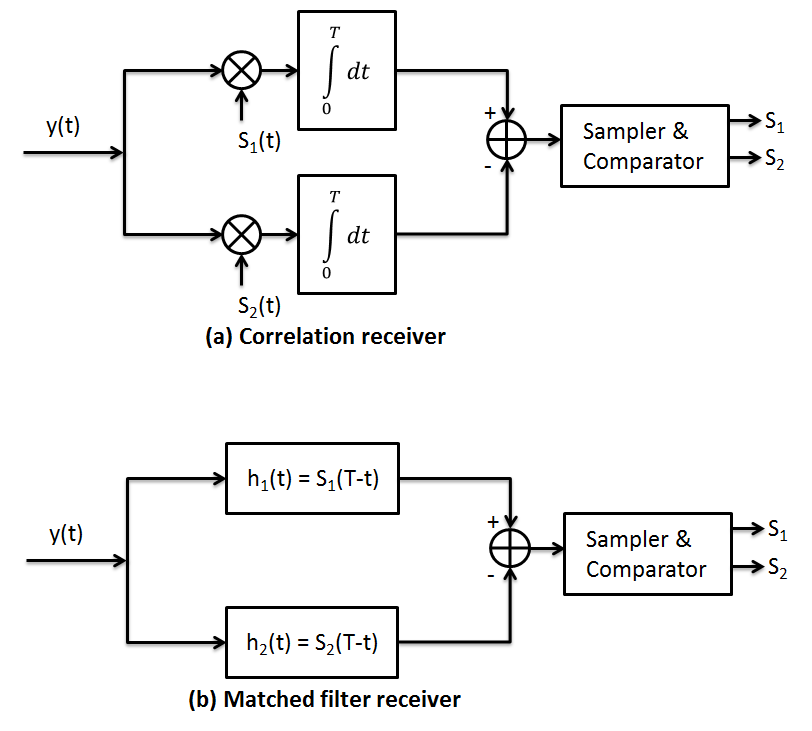
\includegraphics[width=0.75\linewidth]{images/MyBlockDiagrams.png} 
	\caption{Block diagrams for (a) A Correlation Receiver and (b) A Matched Filter Receiver\,\cite{J.Das1986}.}
   \label{BlockDiagrams}
\end{figure}

\begin{figure}
  \centering
	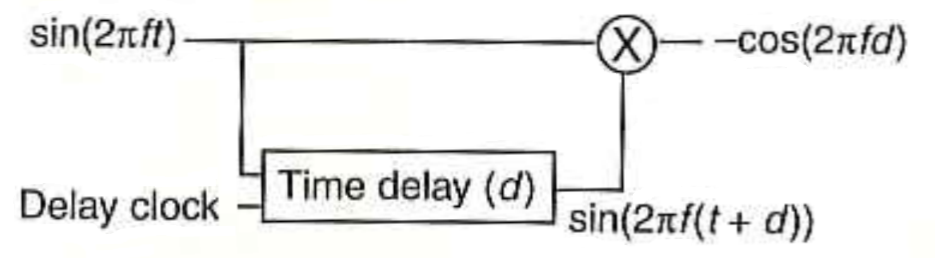
\includegraphics[width=0.75\linewidth]{images/TimeDelayCorrelator.png} 
	\caption{Block Diagram of a time delay correlator\,\cite{Seguine2006}.}
   \label{TimeDelayCorrelator}
\end{figure}

\section{Filtering}
Much like the correlation demodulation approach, a filter based demodulator operates on knowing the expected frequencies in the FSK signal. For our case of 1200Hz and 2200Hz frequencies, a filter will be set and centered about each one of these frequencies. The input signal is passed to each one of these narrow band pass filters and then the power of each of the signals out of the filters is fed to a comparator. The stronger of the two frequencies is the one that must have been present in the original signal\,\cite{Watson1980}. One example of a filter that can be used is a Finite Impulse Response (FIR) Filter. The block diagram for this approach can be seen in Figure \ref{BlockDiagrams}, and the general structure is very similar to correlation. This method seems to be prevalent in both hardware and software based approaches. For instance, if one examines the schematic for the PK-232 MBX, two parallel filters can be seen\,\cite{Inc.2001}. Rossopoulos's Packet Engine measures the energy on the two modem frequencies using filters to do the demodulation. Sailer's Sound Modem also uses a matched filter demodulation\,\cite{Sailer1995} whose algorithm was then reused on a micro controller by Holder\,\cite{Holder2012}. Additionally, AMD produced an FSK Modem chip that used digital filtering for demodulation\,\cite{Devices1989}. All of these independent uses make this look like the most prominent approach for demodulation.

\subsection{Discrete Fourier Transform}
One example of a digital filter is a Discrete Fourier Transform (DFT). A discrete Fourier Transform is one implementation of Fourier Transform that is executed on discrete samples similar to what is present in a digital audio file. Once a Fourier transform has been applied on a signal the output is a relative power versus frequency. With this data, whichever frequency (either 1200Hz or 2200Hz) is more prominent is the symbol which must be present in the bit period, and hence can be used for the demodulation; however, Fourier Transforms are computationally intensive.

\subsection{Goertzel Algorithm}
Computing a discrete Fourier transform is more reasonable computationally than a full Fourier transform, which is a continuous integral as opposed to having discrete terms\,\cite{WikipediaFT}. However, even the results from the DFT have more data than is needed to do the demodulation since the results will be a spectrum of powers over a range of frequencies\,\cite{WikipediaDFT,WikipediaFFT}. A more simplified and specific approach can be used. The Goertzel Algorithm evaluates the coefficients and corresponding powers of the individual frequencies of 1200Hz and 2200Hz\,\cite{WikipediaGA,Elmenreich2011}. This approach, sometimes called a Goertzel Filter, means that no additional computation is wasted on computing frequency power data that is not relevant, making it faster and a vast simplification to the DFT\,\cite{SanjitK1993}.

\section{Phase Locked Loop}
Another option for determining the frequencies present in the original data carrying signal, and hence the actual data in the signal, is to use a Phase-Locked Loop (PLL)\,\cite{Akoum,Perrott2009,Lutus2011}. There are a few different approaches for utilizing a phase locked loop. The basic idea is that there is an internal oscillator and the input (the received signal) is used to influence this oscillator\,\cite{Gaeddert2013} . The input signal and the reference oscillator signal are integrated and this output is used for feedback to the internal oscillator (hence the loop portion of PLL)\,\cite{Roppel}. The convenient thing about monitoring the phase of the signal so closely and being able to stay locked onto it is that the frequency must also be known and this is the portion that is really of interest. A block diagram of a phase locked loop can be seen in Figure \ref{PLLBlockDiagram}. There is a chip produced by Exar that does FSK demodulation and tone detection using a PLL, for which the model number is XR-2211A\,\cite{EXAR1997}. A circuit diagram of using the XR-2211A for Bell 202 can be seen in Figure \ref{XR2211Circuit} which also shows some of the primary items needed for a PLL including the phase detection (integrator) and the VCO (Voltage Controlled Oscillator).

\begin{figure}
  \centering
	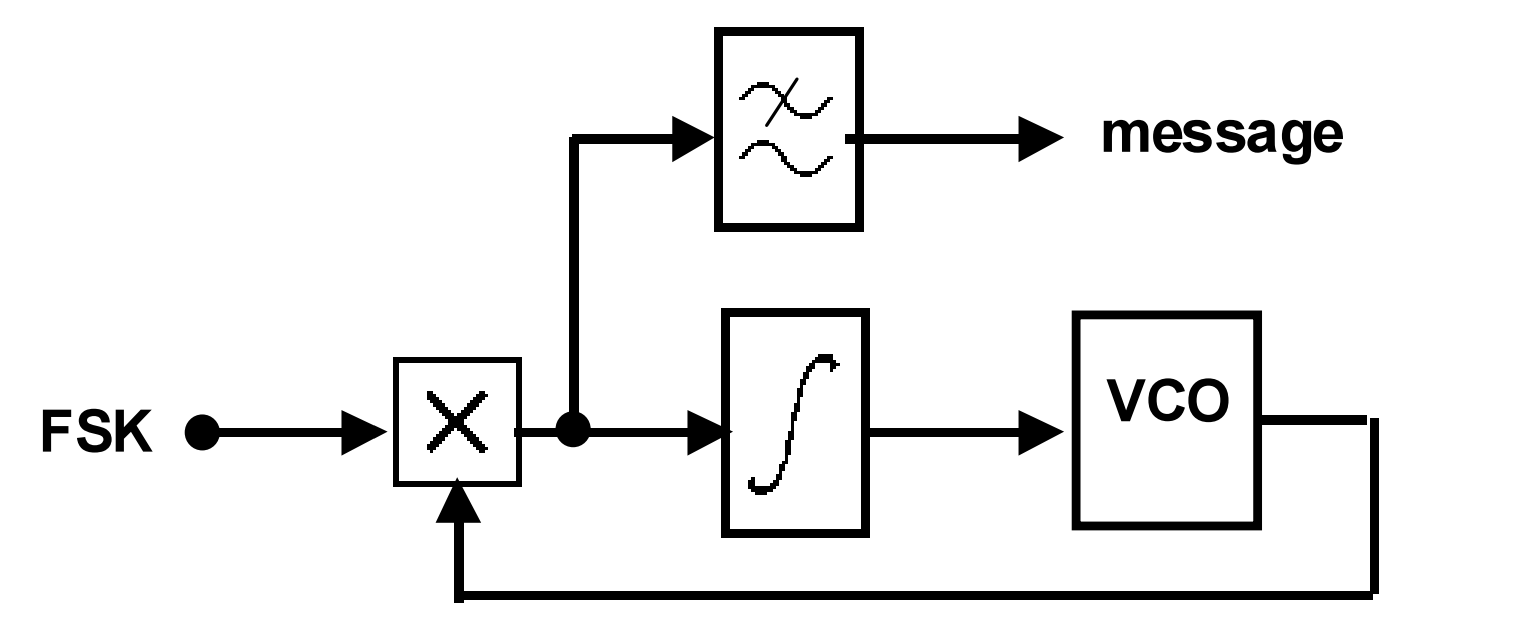
\includegraphics[width=0.75\linewidth]{images/PLLBlockDiagram.PNG} 
	\caption{Block diagram of a PLL demodulator\,\cite{Roppel}.}
   \label{PLLBlockDiagram}
\end{figure}
\begin{figure}
  \centering
	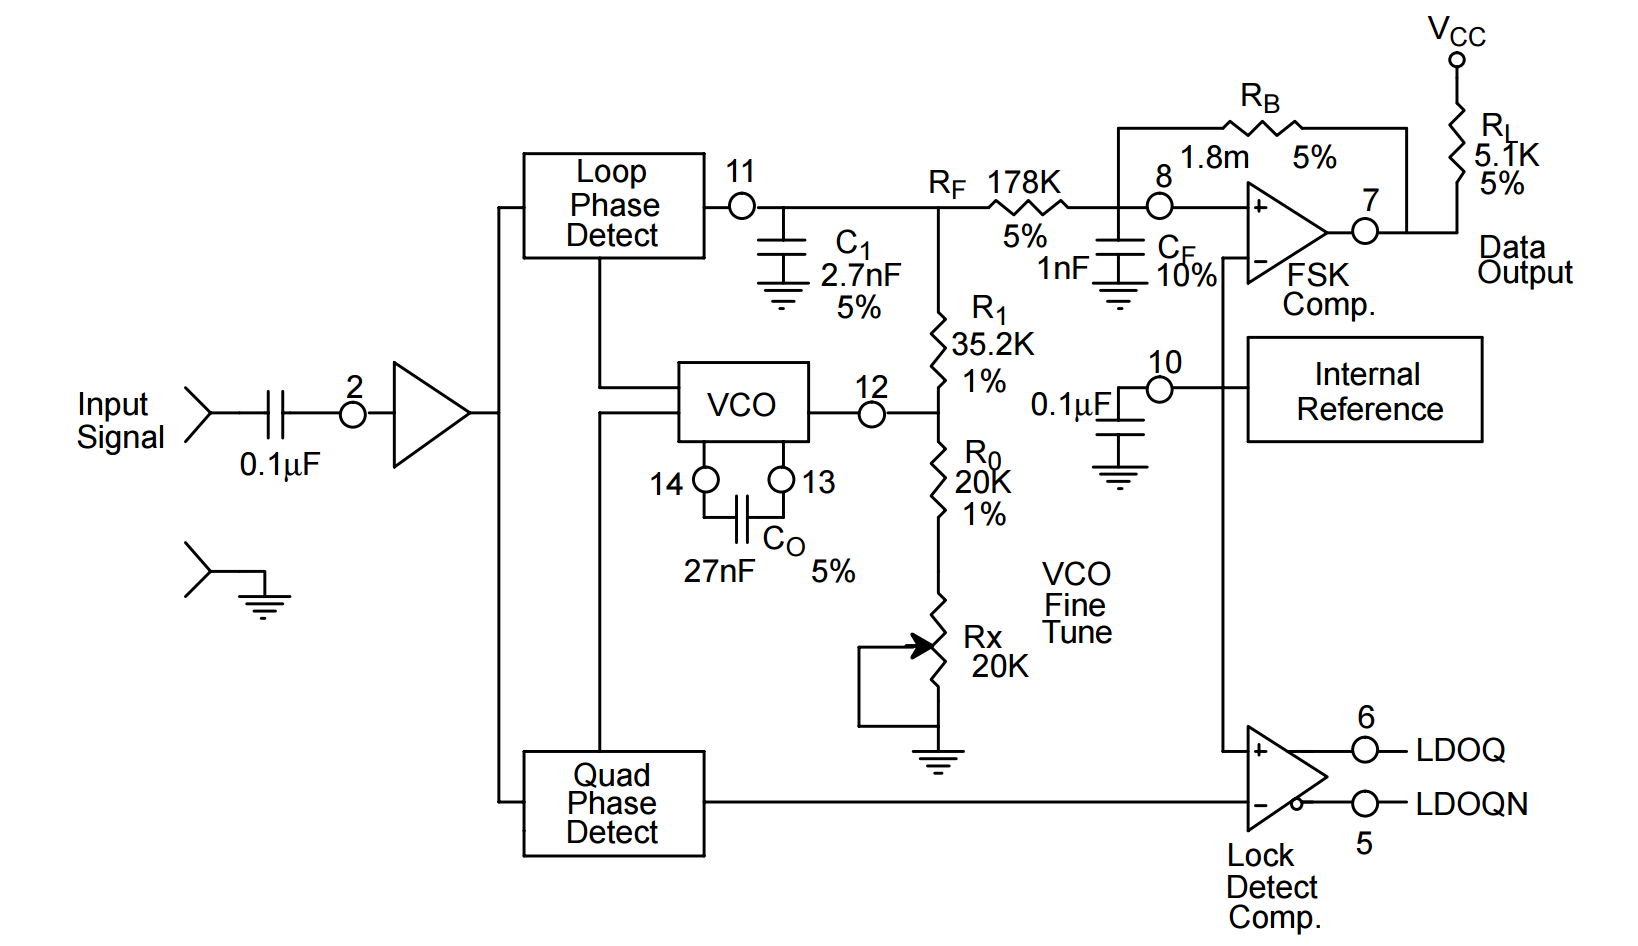
\includegraphics[width=0.75\linewidth]{images/XR2211Circuit.PNG} 
	\caption{Circuit connection for FSK Decoding of Bell 202 Format using an Exar XR-2211A\,\cite{EXAR1997}.}
   \label{XR2211Circuit}
\end{figure}

\section{Additional Benefits of Software Based Decoding}
Software is flexible. As Bergquist mentioned, it was only a matter of time before hams developed a bond between computers and radios using TNCs and it is time to take it a step further and leverage the capabilities of a computer even more\,\cite{Bergquist2001}. Any one of the aforementioned algorithms can be used on the same hardware without having to add additional discrete components, new Integrated Circuits (ICs), or make modifications to a Printed Circuit Board (PCB). There are a two benefits of using software instead of dedicated hardware that this research will investigate; first exhaustive search of a signal through the use of buffers, and second, the ability to be able to run multiple of these demodulation approaches in parallel.

\subsection{Exhaustive Search of Incoming Signal}
Using software the input signal can be buffered in the program and then searched for a signal. Since there is not a separate data and clock signal, there could be a case when the clocking is improperly selected. Using an approach of buffering data that may contain a valid packet, the software can step through the data trying every possible clocking option.

\subsection{Taking Advantage of Parallel Demodulation}
Another advantage of using software for decoding these AFSK signals is being able to apply multiple demodulation techniques. Once the data is collected and converted to a digital form there is no reason, other than computation limitations of the host computer, not to run multiple algorithms in parallel in order to be able to demodulate the maximum number of packets possible. Although there are packets that every algorithm is able to decode, there are also those that some approaches can decode while others can not. Through using multiple demodulators in parallel and de-duplicating the results even more packets can be correctly decoded.